\documentclass[
	11pt,
]{beamer}

% Specifies where to look for included images (trailing slash required)

\usepackage{booktabs} % Allows the use of \toprule, \midrule and \bottomrule for better rules in tables

%----------------------------------------------------------------------------------------
%	SELECT LAYOUT THEME
%----------------------------------------------------------------------------------------

% Beamer comes with a number of default layout themes which change the colors and layouts of slides. Below is a list of all themes available, uncomment each in turn to see what they look like.

%\usetheme{default}
%\usetheme{AnnArbor}
%\usetheme{Antibes}
%\usetheme{Bergen}
%\usetheme{Berkeley}
%\usetheme{Berlin}
%\usetheme{Boadilla}
%\usetheme{CambridgeUS}
%\usetheme{Copenhagen}
%\usetheme{Darmstadt}
%\usetheme{Dresden}
%\usetheme{Frankfurt}
%\usetheme{Goettingen}
%\usetheme{Hannover}
%\usetheme{Ilmenau}
%\usetheme{JuanLesPins}
%\usetheme{Luebeck}
\usetheme{Madrid}
%\usetheme{Malmoe}
%\usetheme{Marburg}
%\usetheme{Montpellier}
%\usetheme{PaloAlto}
%\usetheme{Pittsburgh}
%\usetheme{Rochester}
%\usetheme{Singapore}
%\usetheme{Szeged}
%\usetheme{Warsaw}

%----------------------------------------------------------------------------------------
%	SELECT COLOR THEME
%----------------------------------------------------------------------------------------

% Beamer comes with a number of color themes that can be applied to any layout theme to change its colors. Uncomment each of these in turn to see how they change the colors of your selected layout theme.

%\usecolortheme{albatross}
%\usecolortheme{beaver}
%\usecolortheme{beetle}
%\usecolortheme{crane}
%\usecolortheme{dolphin}
%\usecolortheme{dove}
%\usecolortheme{fly}
%\usecolortheme{lily}
%\usecolortheme{monarca}
%\usecolortheme{seagull}
%\usecolortheme{seahorse}
%\usecolortheme{spruce}
%\usecolortheme{whale}
%\usecolortheme{wolverine}

%----------------------------------------------------------------------------------------
%	SELECT FONT THEME & FONTS
%----------------------------------------------------------------------------------------

% Beamer comes with several font themes to easily change the fonts used in various parts of the presentation. Review the comments beside each one to decide if you would like to use it. Note that additional options can be specified for several of these font themes, consult the beamer documentation for more information.

 % Typeset using the default sans serif font
\usefonttheme{professionalfonts}
%\usefonttheme{serif} % Typeset using the default serif font (make sure a sans font isn't being set as the default font if you use this option!)
%\usefonttheme{structurebold} % Typeset important structure text (titles, headlines, footlines, sidebar, etc) in bold
%\usefonttheme{structureitalicserif} % Typeset important structure text (titles, headlines, footlines, sidebar, etc) in italic serif
%\usefonttheme{structuresmallcapsserif} % Typeset important structure text (titles, headlines, footlines, sidebar, etc) in small caps serif

%------------------------------------------------

%\usepackage{mathptmx} % Use the Times font for serif text
%\usepackage{palatino} % Use the Palatino font for serif text
\usepackage[utf8]{inputenc} % allow utf-8 input
\usepackage[T1]{fontenc}    % use 8-bit T1 fonts
\usepackage{hyperref}       % hyperlinks
\usepackage{url}            % simple URL typesetting
\usepackage{booktabs}       % professional-quality tables
\usepackage{amsfonts}       % blackboard math symbols
\usepackage{nicefrac}       % compact symbols for 1/2, etc.
\usepackage{microtype}      % microtypography
\usepackage{lipsum}
\usepackage{fancyhdr}       % header
\usepackage{graphicx}       % graphics
\usepackage{physics}
\usepackage{xcolor}
\usepackage{amsmath}
\usepackage{algorithm}
\usepackage{algpseudocode}

%\usepackage{helvet} % Use the Helvetica font for sans serif text
 % Use the Open Sans font for sans serif text
%\usepackage[default]{FiraSans} % Use the Fira Sans font for sans serif text
%\usepackage[default]{lato} % Use the Lato font for sans serif text

%----------------------------------------------------------------------------------------
%	SELECT INNER THEME
%----------------------------------------------------------------------------------------

% Inner themes change the styling of internal slide elements, for example: bullet points, blocks, bibliography entries, title pages, theorems, etc. Uncomment each theme in turn to see what changes it makes to your presentation.

%\useinnertheme{default}
\useinnertheme{circles}
%\useinnertheme{rectangles}
%\useinnertheme{rounded}
%\useinnertheme{inmargin}

%----------------------------------------------------------------------------------------
%	SELECT OUTER THEME
%----------------------------------------------------------------------------------------

% Outer themes change the overall layout of slides, such as: header and footer lines, sidebars and slide titles. Uncomment each theme in turn to see what changes it makes to your presentation.

%\useoutertheme{default}
%\useoutertheme{infolines}
%\useoutertheme{miniframes}
%\useoutertheme{smoothbars}
%\useoutertheme{sidebar}
%\useoutertheme{split}
%\useoutertheme{shadow}
%\useoutertheme{tree}
%\useoutertheme{smoothtree}

%\setbeamertemplate{footline} % Uncomment this line to remove the footer line in all slides
%\setbeamertemplate{footline}[page number] % Uncomment this line to replace the footer line in all slides with a simple slide count

%\setbeamertemplate{navigation symbols}{} % Uncomment this line to remove the navigation symbols from the bottom of all slides

%----------------------------------------------------------------------------------------
%	PRESENTATION INFORMATION
%----------------------------------------------------------------------------------------
\setbeamertemplate{itemize item}[ball]
\setbeamertemplate{enumerate item}[ball]
\title[Design and Analysis of Algorithms]{Complete search - Backtracking} % The short title in the optional parameter appears at the bottom of every slide, the full title in the main parameter is only on the title page

% \subtitle{and the Exploding and Vanishing Gradient Problems} % Presentation subtitle, remove this command if a subtitle isn't required

\author[Group 2]{
                    Le Gia Khang \and 21522189 \\
                    Nguyen Hoang Tan \and 21521413 \\} % Presenter name(s), the optional parameter can containa shortened version to appear on the bottom of every slide, while the main parameter will appear on the title slide

\institute[UIT]{\fontsize{10}{12}\selectfont \textbf{University of Information Technology} \\ \smallskip \textit{}} % Your institution, the optional parameter can be used for the institution shorthand and will appear on the bottom of every slide after author names, while the required parameter is used on the title slide and can include your email address or additional information on separate lines

\date[\today]{ \\ \today} % Presentation date or conference/meeting name, the optional parameter can contain a shortened version to appear on the bottom of every slide, while the required parameter value is output to the title slide

%----------------------------------------------------------------------------------------

\begin{document}

%----------------------------------------------------------------------------------------
%	TITLE SLIDE
%----------------------------------------------------------------------------------------
\setcounter{tocdepth}{1}
\begin{frame}
	\titlepage % Output the title slide, automatically created using the text entered in the PRESENTATION INFORMATION block above
\end{frame}

%----------------------------------------------------------------------------------------
%	TABLE OF CONTENTS SLIDE
%----------------------------------------------------------------------------------------

% The table of contents outputs the sections and subsections that appear in your presentation, specified with the standard \section and \subsection commands. You may either display all sections and subsections on one slide with \tableofcontents, or display each section at a time on subsequent slides with \tableofcontents[pausesections]. The latter is useful if you want to step through each section and mention what you will discuss.

\begin{frame}
	\frametitle{References}
	The contents of this document are taken mainly from the follow sources:
	\begin{itemize}
		\item Rina Dechter and Daniel Frost, Backtrackging algorithms for constraint satisfaction problems 
		\item Pter van Beek, Chapter 4 - Backtracking Search Algorithms
	\end{itemize}

	%\footnote[2]{https://arxiv.org/pdf/1211.5063.pdf}
	%\footnote[3]{https://www.researchgate.net/profile/Y-Bengio/publication/5583935_Learning_long-term_dependencies_with_gradient_descent_is_difficult/links/546b702d0cf2397f7831c03d/Learning-long-term-dependencies-with-gradient-descent-is-difficult.pdf}
\end{frame}
\begin{frame}
	\frametitle{Table of Contents} % Slide title, remove this command for no title
	
	\tableofcontents % Output the table of contents (all sections on one slide)
	%\tableofcontents[pausesections] % Output the table of contents (break sections up across separate slides)
\end{frame}

%----------------------------------------------------------------------------------------
%	PRESENTATION BODY SLIDES
%----------------------------------------------------------------------------------------

\section{Preliminaries} % Sections are added in order to organize your presentation into discrete blocks, all sections and subsections are automatically output to the table of contents as an overview of the talk but NOT output in the presentation as separate slides
\begin{frame}
	\frametitle{Table of Contents}

	\tableofcontents[currentsection]
\end{frame}
%------------------------------------------------
\subsection{Constraint satisfaction problems (CSPs)}
\begin{frame}
    \frametitle{Constraint satisfaction problems (CSPs)}

    \begin{itemize}
        \item A special subset of search problems.
        \bigskip
        \item State is defined by \textcolor{red}{variables \textbf{$X_i$}}  with values from a \textcolor{red}{domain \textbf{$D$}} (sometimes \textbf{$D$} depends on \textbf{$i$})
        \bigskip
        \item Goal test is a \textcolor{red}{set of constraints} specifying allowable combinations of values for subsets of variables
        \bigskip
    \end{itemize}
    \begin{figure}
        \centering
        \begin{minipage}{.5\textwidth}
          \centering
          
\includegraphics[scale=0.2]{Figs/csp_1.png}
        \end{minipage}%
        \begin{minipage}{.5\textwidth}
          \centering
          
\includegraphics[scale=0.2]{Figs/csp_2.png}
        \end{minipage}
        \end{figure}
\end{frame}

\begin{frame}
    \frametitle{Constraint satisfaction problems (CSPs)}

    \begin{block}{Definition}
        A constraint satisfaction problem (CSP) is a tuple (X,D,C) where:
        \begin{itemize}
            \item $X=\{x_1,x_2,…,x_n\}$ is the set of variables.
            \item $D=\{d_1,d_2,…,d_n\}$ is the set of domains.
            \item $C=\{c_1,c_2,…,c_n\}$ is a set of constraints.
        \end{itemize}
    \end{block}
    \bigskip
    For example, $x,y,z \in \{0,1\}, x + y = z$ is a CSP where:
    \begin{itemize}
        \item Variables are: $x,y,z$
        \item Domains are: $d_x = d_y = d_z = \{0,1\}$
        \item There is a single constraint: $x + y = z$
    \end{itemize}
\end{frame}
\section{Backtracking Algotithm}
\begin{frame}
    \frametitle{Table of Contents}
    \tableofcontents[currentsection]
\end{frame}
\subsection{Brute-force}
\begin{frame}
	\frametitle{Brute-force Approach}
	\begin{itemize}
		\item Brute-force is a simple and naive algorithmic approach to solving problems that involves exhaustively checking all possible solutions. 
	\bigskip
		\item It is typically used when the problem size is small and the search space is manageable.
	\bigskip
        \item It can also be used in combination with other techniques, such as pruning or heuristics, to improve their efficiency and effectiveness.
    \bigskip
\end{itemize}
\end{frame}

\subsection{Complete Search - Backtracking}
\begin{frame}
    \frametitle{Complete Search - Backtracking}
    \begin{center}
        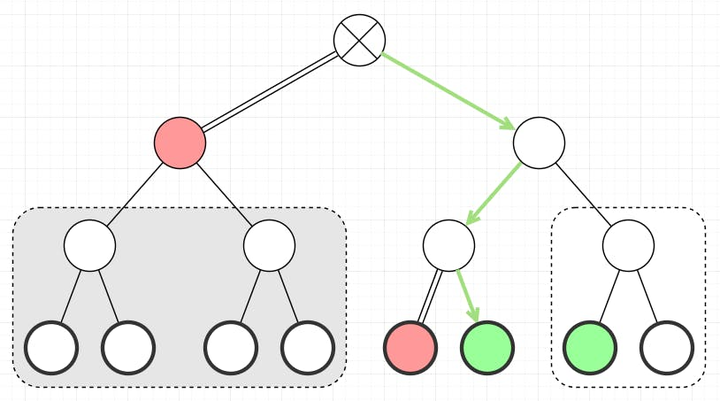
\includegraphics[scale=0.5]{Figs/backtracking.png}
    \end{center}
\end{frame}
\begin{frame}
	\frametitle{Complete Search - Backtracking}
	\begin{itemize}
		\item The basic idea behind backtracking is to recursively build a partial solution by making choices from a set of available options, and then backtrack if the solution fails to satisfy the constraints. 
		\bigskip
		\item The algorithm explores the search space depth-first, which means that it goes as far as possible along each branch of the search tree before backtracking to the previous decision point and exploring another branch.
		\bigskip
        \item if a node in the search tree does not lead to a solution, it is considered a deadend and its subtree can be pruned. 
	\end{itemize}
\end{frame}
\begin{frame}
	\frametitle{Complete Search - Backtracking}
    \begin{figure}
        \centering
        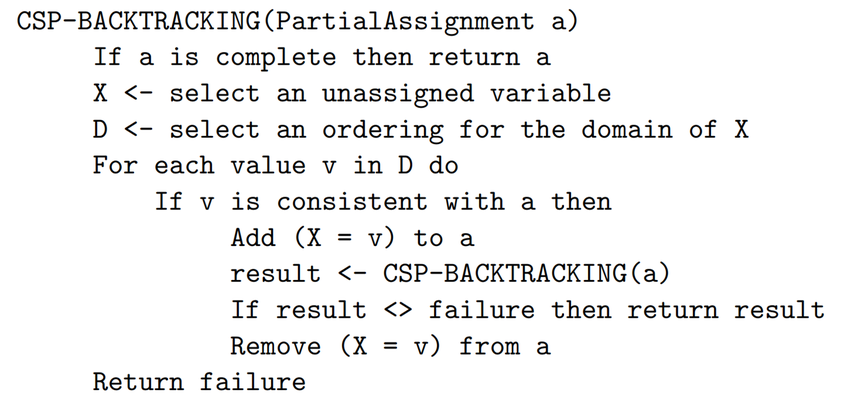
\includegraphics[scale=0.3]{Figs/pcode_1.png}
        \end{figure}
        
\end{frame}
\section{Problems}
\begin{frame}
    \frametitle{Table of Contents}
    \tableofcontents[currentsection]
\end{frame}
\begin{frame}
	\frametitle{N-queens problem}
	The N-Queens problem is a classic problem in computer science and mathematics that involves placing N chess queens on an N x N chessboard such that no two queens attack each other.
    \bigskip 
    \begin{figure}
        \centering
        \begin{minipage}{.5\textwidth}
          \centering
          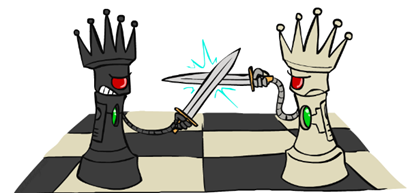
\includegraphics[scale=0.4]{Figs/n_queens_1.png}
        \end{minipage}%
        \begin{minipage}{.5\textwidth}
          \centering
          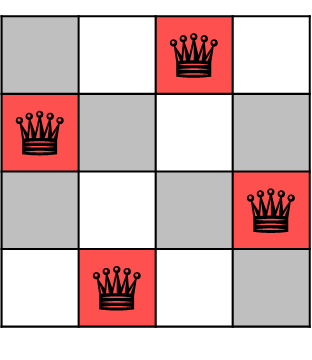
\includegraphics[scale=0.4]{Figs/n_queens_2.png}
        \end{minipage}
        \end{figure}
\end{frame}



\begin{frame}
	\frametitle{Knapsack}
	The Knapsack problem involves packing a knapsack with items of different weights and values. The goal is to maximize the value of the items in the knapsack while keeping the total weight of the knapsack below a certain limit.
    \begin{figure}
        \centering
        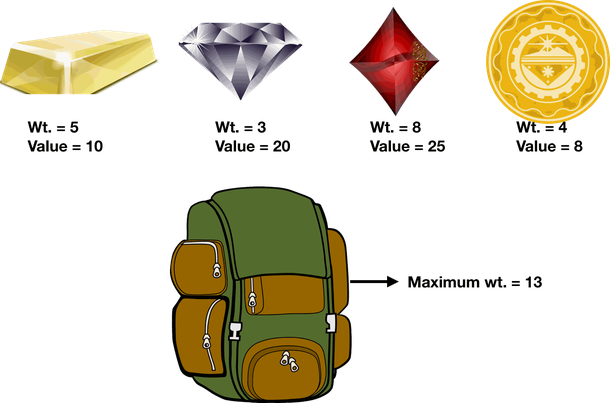
\includegraphics[scale=0.3]{Figs/knapsack.png}
    \end{figure}
\end{frame}

\section{Optimization}
\begin{frame}
    \frametitle{Table of Contents}
    \tableofcontents[currentsection]
\end{frame}

\begin{frame}
    \frametitle{Benefits and Drawbacks of Backtracking}
    \large{\textcolor{blue}{\textbf{Benefits}}}
    \bigskip
	\begin{itemize}
		\item Backtracking is a more intelligent and efficient way of searching through large solution spaces than brute-force;
		\bigskip
		\item Backtracking problems are very intuitive to code;
	\end{itemize}
	\bigskip
	\large{\textcolor{red}{\textbf{Drawbacks}}}
    \bigskip
	\begin{itemize}
		\item In the worst case where all possible solutions must be explored, Backtracking has the same worst-case time \& space complexity as Brute-force;
		\bigskip
		\item Backtracking is complete but not guaranteed to find optimal solution, or just sub-optimal;
	\end{itemize}
    
\end{frame}

\begin{frame}
    \frametitle{Improvements to backtracking}
    \begin{columns}
    \begin{column}{0.5\textwidth}
        \begin{itemize}
            \item Backtracking usually suffers from thrashing, namely, rediscovering the same inconsistencies and the same partial successes during search.
            \bigskip
            \item Efficient cures for such behavior in all cases are unlikely, since the problem is NP-hard.
        \end{itemize}
    \end{column}
    \begin{column}{.5\textwidth}
        \begin{figure}[h]
            \centering
            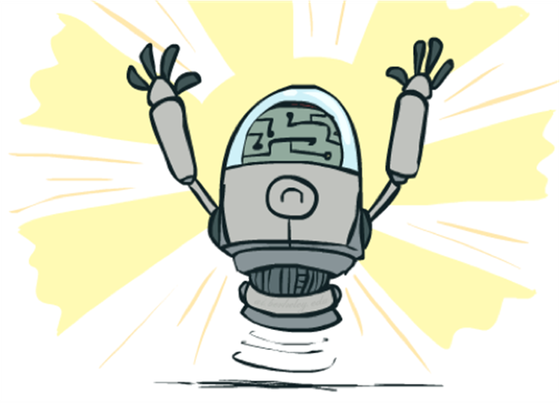
\includegraphics[scale=0.3]{Figs/improve.png}
        \end{figure}
    \end{column}
\end{columns}
\end{frame}

\begin{frame} 
    \frametitle{Filtering}
    \begin{figure}[h]
        \centering
        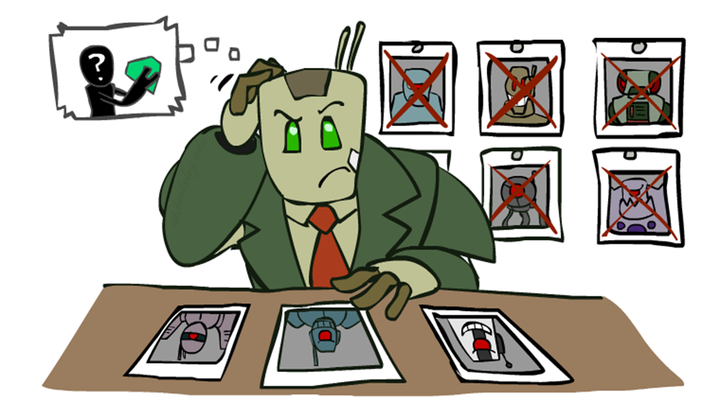
\includegraphics[width=\textwidth]{Figs/filtering.png}
    \end{figure}
\end{frame}
\begin{frame}
    \frametitle{Ordering}
    \begin{figure}[h]
        \centering
        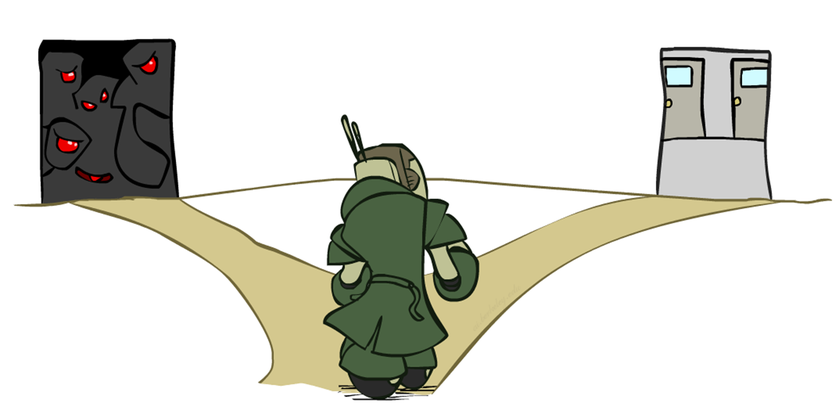
\includegraphics[width=\textwidth]{Figs/ordering.png}
    \end{figure}
\end{frame}
\end{document} 